\documentclass[tikz,border=10pt,12pt,x11names]{standalone}
\usepackage{tikz}
\usetikzlibrary{circuits.logic.US} % TiKZ Library for US Logic Circuits.
\begin{document}

	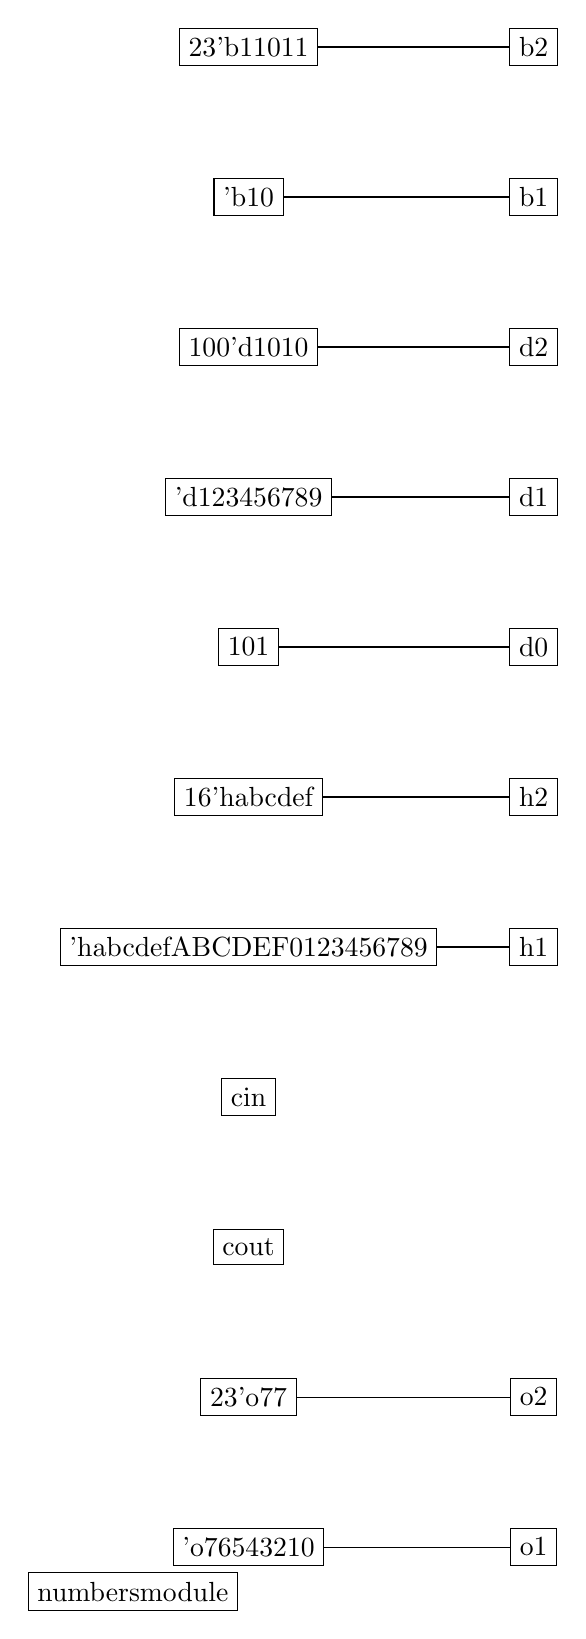
\begin{tikzpicture}[circuit logic US,
						tiny circuit symbols,
						every circuit symbol/.style={
						fill=white,draw}]

		\node[draw] at (-2.0bp,2.0bp) {numbersmodule};

		\node[draw, inputs={n}] (o1) at (142.29bp,18.0bp) {o1};
		\node[draw, inputs={n}] (o2) at (142.29bp,72.0bp) {o2};
		\node[draw] (cout) at (39.646bp,126.0bp) {cout};
		\node[draw] (cin) at (39.646bp,180.0bp) {cin};
		\node[draw, inputs={n}] (h1) at (142.29bp,234.0bp) {h1};
		\node[draw] (nodeº19) at (39.646bp,288.0bp) {16'habcdef};
		\node[draw, inputs={n}] (h2) at (142.29bp,288.0bp) {h2};
		\node[draw, inputs={n}] (d0) at (142.29bp,342.0bp) {d0};
		\node[draw, inputs={n}] (d1) at (142.29bp,396.0bp) {d1};
		\node[draw, inputs={n}] (d2) at (142.29bp,450.0bp) {d2};
		\node[draw, inputs={n}] (b1) at (142.29bp,504.0bp) {b1};
		\node[draw, inputs={n}] (b2) at (142.29bp,558.0bp) {b2};
		\node[draw] (nodeº12) at (39.646bp,504.0bp) {'b10};
		\node[draw] (nodeº11) at (39.646bp,342.0bp) {101};
		\node[draw] (nodeº14) at (39.646bp,396.0bp) {'d123456789};
		\node[draw] (nodeº13) at (39.646bp,18.0bp) {'o76543210};
		\node[draw] (nodeº16) at (39.646bp,558.0bp) {23'b11011};
		\node[draw] (nodeº15) at (39.646bp,234.0bp) {'habcdefABCDEF0123456789};
		\node[draw] (nodeº18) at (39.646bp,450.0bp) {100'd1010};
		\node[draw] (nodeº17) at (39.646bp,72.0bp) {23'o77};

		\draw (nodeº19.east) -- ++(right:3mm) |- (h2);
		\draw (nodeº12.east) -- ++(right:3mm) |- (b1);
		\draw (nodeº11.east) -- ++(right:3mm) |- (d0);
		\draw (nodeº14.east) -- ++(right:3mm) |- (d1);
		\draw (nodeº13.east) -- ++(right:3mm) |- (o1);
		\draw (nodeº16.east) -- ++(right:3mm) |- (b2);
		\draw (nodeº15.east) -- ++(right:3mm) |- (h1);
		\draw (nodeº18.east) -- ++(right:3mm) |- (d2);
		\draw (nodeº17.east) -- ++(right:3mm) |- (o2);

	\end{tikzpicture}

\end{document}